% ============================================================================
% Title: Corrosion in structural materials
% Author: Nathaniel Thomas
% Affiliation:  Texas A&M University, Department of Nuclear Engineering
% Email:        nathaniel@tamu.edu
% Date Created: 3/15/2026
% Version:      1.0
%
% Description:
%   A .tex source file for a literature review discussing corrosion
%   in structural materials.
%
% =============================================================================

\section{Corrosion in Structural Materials}
\label{sec: corrosion}

The highly corrosive properties of both the hydrofluorinating reagents and
the molten salt itself requires a balance between process safety and cost
management. High nickel alloys are far more resistant to corrosion by both
than stainless steels; however, they are also far more expensive
\cite{rev49}. This means that for practical applications, an acceptable
rate of corrosion needs to be established. \par

\subsection{Corrosion Due to Hydrofluorinating Reagents}
\label{sec: corrosion due to hf}

The corrosion mechanism of structural metals by HF is shown by
\Cref{eq: metal oxidation}
. Corrosion occurs by the fluorination of pure metals to metal fluorides,
which can be more easily dissolved into the salt solution.
Both \ch{HF-H2} sparging and \ch{NH4HF2} baking use \ch{HF} as the primary
hydrofluorinating agent. Reversing the directions of
% Equations 9, 10, and 13 TODO
\Cref{eq: O2 to H2O,eq: OH to H2O,eq: S to H2S}
also show that \ch{HF} is produced as a by-product of salt contamination.
\Cref{fig: fluorides gibbs energy}
shows the Gibbs free energy of formation for various elemental metal
fluorides.
\par

\begin{figure}
  \centering
  \includegraphics[width=0.6\textwidth]{./assets/review/figures/fluorides
  gibbs energy.pdf}
  \caption{Gibbs Free Energy of Fluorination of Various Elemental
  Metals \cite{rev33}.}
  \label{fig: fluorides gibbs energy}
\end{figure}

\ch{NF3} corrodes structural metals via the same mechanism as
\ch{HF}: fluorination; however, as stated previously, it is more aggressive
than \ch{HF} at elevated temperatures \cite{rev31}. No corrosion data exists
for \ch{NF3} or any analogous gas, such as fluorine, near expected process
temperatures. This is likely due to the extreme health risks and financial
costs associated with running such an experiment. \par

Because their fluorination potential is higher than that of \ch{Ni},
\ch{Cr} and \ch{Fe} are more easily corroded in a fluorinating environment
and should therefore be reduced as much as possible. \ch{Cr} has an especially
high fluorination potential, causing it to be targeted for attack first
(if present) for most applicable alloys
\cite{rev24,rev33,rev34,rev38,rev50,rev51}.
This high fluorination potential can be and counteracted by diluting the
fluorinating agent with a reducing gas, namely \ch{H2}. The effects of a high
fluorination potential can also be reversed by dropping the fluorination
potential of the salt mix, by removing excess fluorine ions from
the mix, using a reducing agent such as an active metal or \ch{H2} sparging.
\par

\subsection{Embrittlement Due to Hydrogen}
\label{sec: embrittlement}

Although not a direct contributor to corrosion, exposure to \ch{H2} can
cause embrittlement by infiltration into the metal’s grain boundaries.
\ch{H2} can build up along grain boundaries, exerting pressure on and
deforming the grains to reduce ductility and strength. This has the added
effect of increasing the size of grain boundaries, allowing for
increased attack by corrosive agents. For annealed metals, increasing the
\ch{Ni} content tends to increase resistance to hydrogen ingress
affecting structural strength; however, for cold worked metals this trend
is reversed \cite{rev52,rev53}. Increasing the Ni content also causes an
increase in intragranular fracture due to hydrogen embrittlement,
as depicted in \Cref{fig: h2 embrittlement}. \par

\begin{figure}
  \centering
  \includegraphics[width=0.6\textwidth]{./assets/review/figures/h2
  embrittlement.jpg}
  \caption{Microstructure of annealed 316L stainless steel before (a)
    and after (b) 20 hr of cathodic
    hydrogen charging compared to annealed Hastelloy C-276 before (c)
    and after (d) \SI{20}{\hour} of cathodic
  hydrogen charging. \cite{rev53}}
  \label{fig: h2 embrittlement}
\end{figure}

This increase in crack size and frequency in higher Ni alloys would
likely allow for more surface to be
attacked by corrosive agents; however, the higher Ni content likely
more than offsets this through its
higher fluorination resistance. \par

\subsection{Corrosion Due to Molten Salt}
\label{sec: corrosion due to salt}

There are essentially two theorized methods of corrosive attack by molten salt
on structural metals: continuous corrosion due to mass transfer of metals
into the salt and impurities in the salt mix \cite{rev54}. \par

Across the MSRE project, samples of the coolant FLiBe salt were taken to
measure the concentration of \ch{Cr}, \ch{Fe}, and \ch{Ni} dissolved into
the salt as a method of determining the rate of corrosion of the Hastelloy-N
piping by the salt. Analysis of these samples showed that, while there was
an initial spike in metal concentration (thought to be due to reactions
caused by impurities in the salt), the metal concentratileveled off at
\SI{32}{ppm} \ch{Cr}, \SI{64}{ppm} \ch{Fe}, and \SI{20}{ppm} \ch{Ni}. These
values persisted allowing for the time between samples to be taken monthly
and did not spike again until the system had become
contaminated due to atmospheric exposure \cite{rev54}. These findings imply
that continuous corrosion due to mass transfer is minimal, if not
nonexistent, at least for FLiBe with \ch{Ni} alloys. These tests were however
performed in static tests with a constant bulk temperature
throughout. Future testing conducted by Santarini at Oak Ridge National
Lab found that there was sustained corrosion in the MSRE due to the
existence of a temperature gradient in a flowing molten salt loop which
caused an imbalance in the concentration of \ch{Cr^{2+}} in the salt
solution \cite{rev55}. \ch{Cr^{2+}} would build up in colder sections
of the loop, causing more \ch{Cr} to diffuse into the salt at the hotter
sections\cite{rev55}. This phenomenon has since been confirmed
in other experiments, using other metal alloys \cite{rev23,rev35,rev36}. \par

Complete purity is not practically attainable, due to all purification
methods described above being equilibrium reactions. Despite this
corrosion tests have been performed with salt purified to a
reasonable extent. Raiman et al. has compiled results from these tests
into a series of graphs shown in
\Cref{fig:
  corrosion time pure impure,fig:
  corrosion time various materials,fig:
corrosion time various methods} \cite{rev34}. \par

\begin{figure}
  \centering
  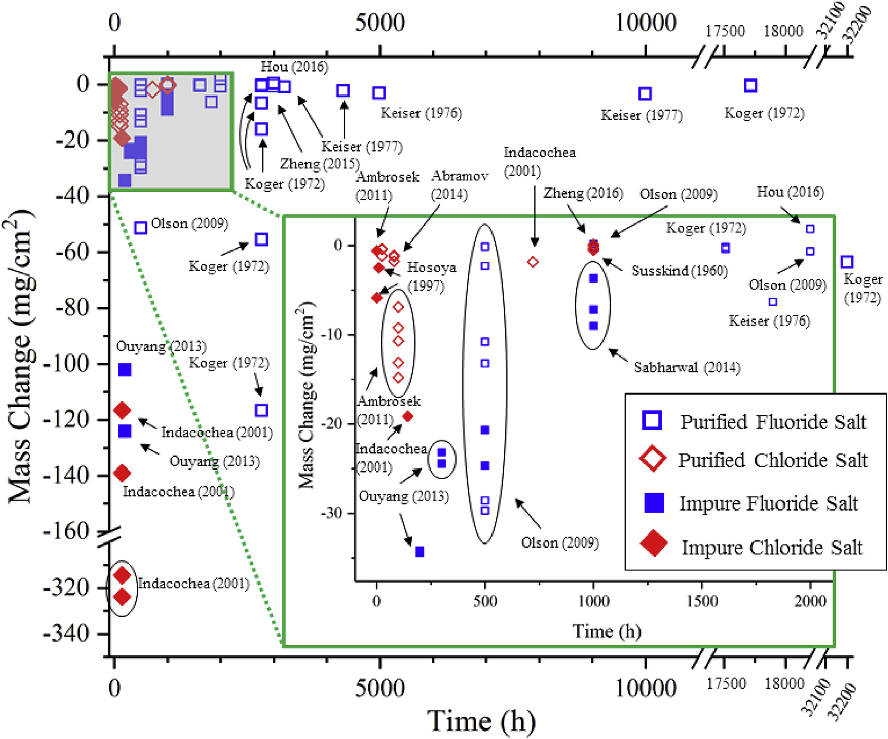
\includegraphics[width=0.6\textwidth]{./assets/review/figures/corrosion_time_pure_impure.pdf}
  \caption{Aggregation of corrosive mass change over time for purified and
    non-purified fluoride and chloride salts across various tests
  \cite{rev34}.}
  \label{fig: corrosion time pure impure}
\end{figure}

\begin{figure}
  \centering
  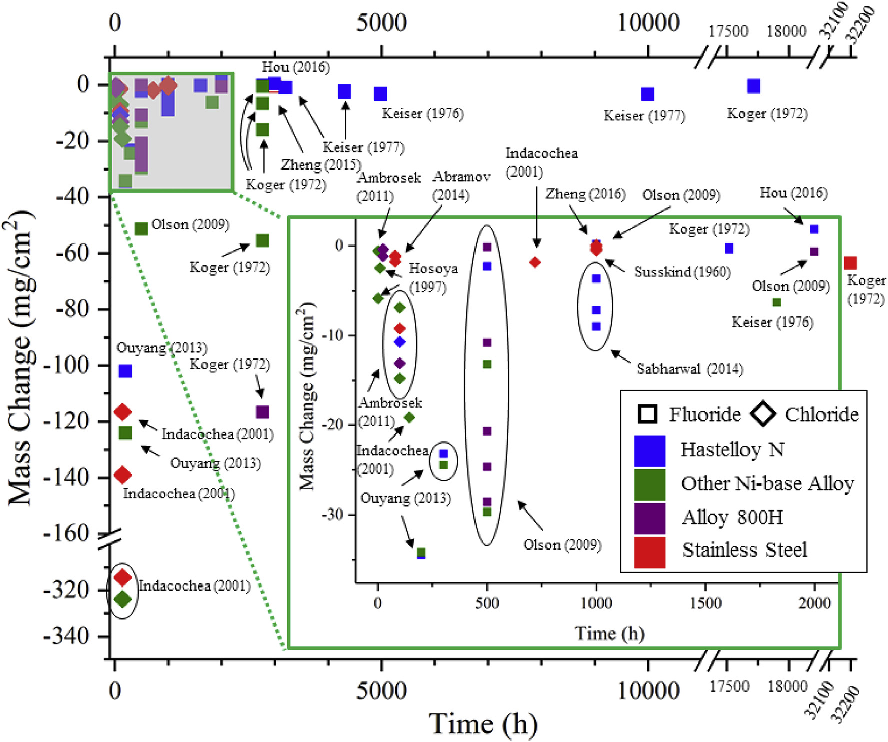
\includegraphics[width=0.6\textwidth]{./assets/review/figures/corrosion_time_various_methods.pdf}
  \caption{Aggregation of corrosive mass change in various materials
    over time for fluoride and chloride salts across various
  materials \cite{rev34}.}
  \label{fig: corrosion time various materials}
\end{figure}

\begin{figure}
  \centering
  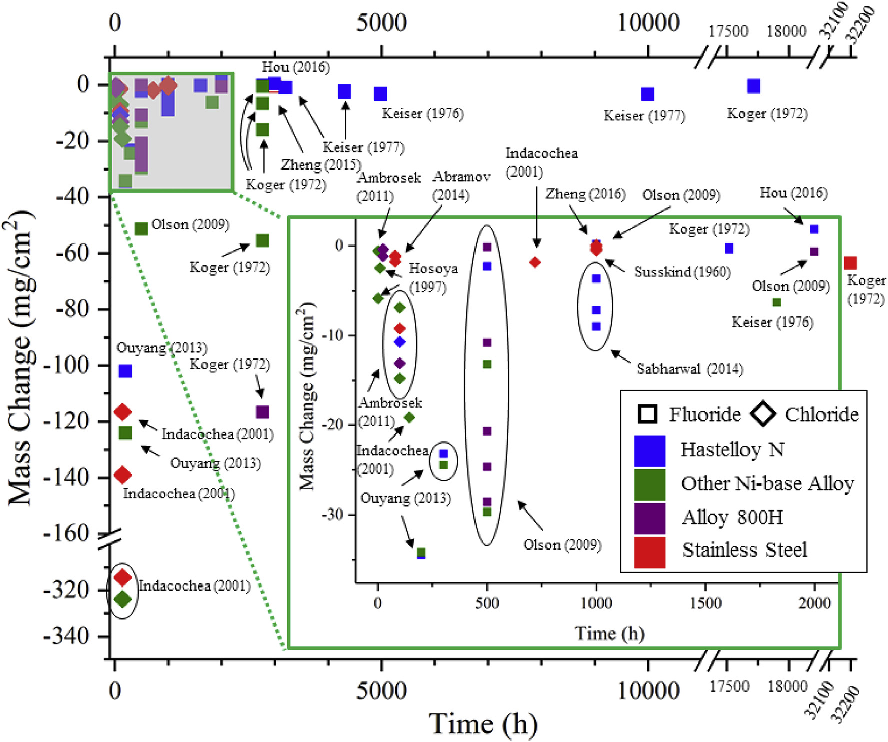
\includegraphics[width=0.6\textwidth]{./assets/review/figures/corrosion_time_various_methods.pdf}
  \caption{Aggregation of corrosive mass change in over time for fluoride
    and chloride salts across various tests using various methods
  \cite{rev34}.}
  \label{fig: corrosion time various methods}
\end{figure}

Results of this aggregation of data show that there is a wide
variance in the reported corrosion rate of
nickel-based alloys and very little data for the corrosion rate of
stainless steels in crucible and loop tests. \par

Just like with other forms of fluorination, \ch{Fe} and
\ch{Cr} will be corroded before \ch{Ni}. The trend for these
metals to be targeted before \ch{Ni} is demonstrated by
\Cref{fig: fluorides gibbs energy}
, where almost pure \ch{Ni} experienced
miniscule corrosion compared to other alloys with higher
\ch{Cr} and \ch{Fe} compositions \cite{rev33}. \par
